\subsection{Hopfield Nets}
\begin{itemize}
	\item A hopfield net is composed of binary threshold units with recurrent connections between them
	\item Recurrent networks of non-linear units are generally very hard to analyze. THey can behave in many different ways:
	\begin{itemize}
		\item Settle to a stable state
		\item Oscillate
		\item Chaotic trajectories (cannot predict future)
	\end{itemize}

	\item John Hopfield realized that if the connections are symmetric, there is a global every function
	\begin{itemize}
		\item Each binary ``configuration'' of the whole network has an energy
		\item The binary threshold decision rule causes the network to a minimum of this energy function
	\end{itemize}

	\subsubsection{The energy function}
	\item The global energy is the sum of many contributions. Each contribution depends on one connection weight and the binary states of two neurons:
		$$E=-\sum_i s_i b_i - \sum_{i<j} s_i s_j w_{ij}$$
	\item This simple quadratic energy function makes it possible for each unit to compute locally how it's state affects the global energy:
		$$\text{Energy gap}=\delta E_i = E(s_i = 0) - E(s_i = 1) = b_i + \sum_j s_j w_{ij}$$
	\item Energy gap is the difference in energy when it is off minus when it is on
	
	\subsubsection{Settling to an energy minimum}
	\item To find an energy minimum in this net, start from a random state and then update units one at a time in random order
	\begin{itemize}
		\item Update each unit to whichever of its two states give the lowest global energy
		\item i.e., use binary threshold units
	\end{itemize}
	\begin{center}
		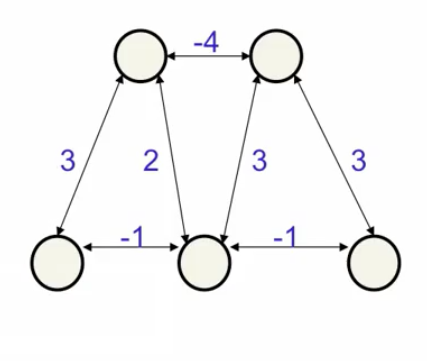
\includegraphics[scale=0.8]{sections/11/min.png}
	\end{center}
	$$-\text{Energy}=\text{goodness}=3$$

	\item A random unit is selected, and the question is asked: What state should that be in, given the current states of all other units?
	\begin{center}
		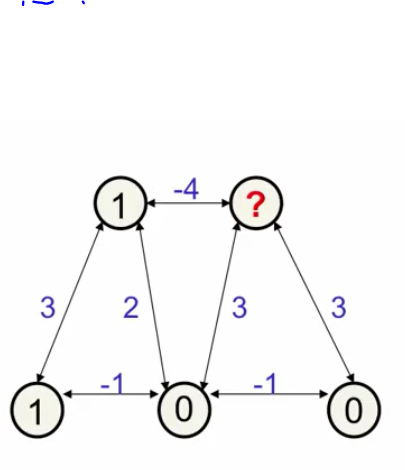
\includegraphics[scale=0.8]{sections/11/picked.png}
	\end{center}
	\begin{center}
		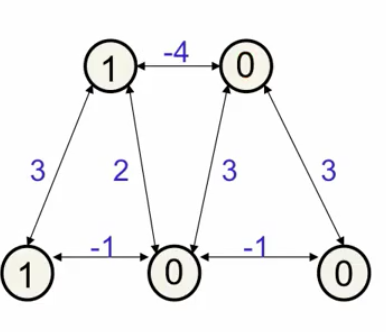
\includegraphics[scale=0.8]{sections/11/off.png}
	\end{center}

	$$-4(1)+3(0)+3(0)=-4<0\to \text{Turn off}$$
	\item Repeat for remaining units

	\subsubsection{A deeper energy minimum}
	\item The net has two triangles in which the three units mostly support each other
	\item Each triangle mostly hates the other triangle (-4 at the top)
	\item The triangle on the left differs from the one on the right by having a weight of 2 where the other one has a weight of 3
	\item So turning on the units in the triangle on the right gives the deepest minimum.
	\begin{center}
		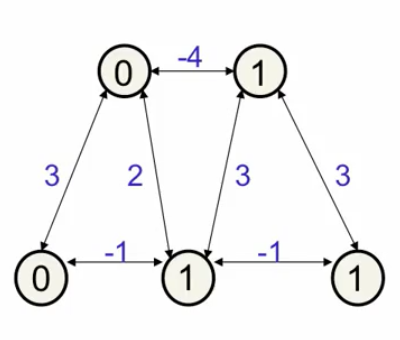
\includegraphics[scale=0.8]{sections/11/deep.png}
	\end{center}

	\subsubsection{Who do the decisions need to be sequential?}
	\item If units make simultaneous decisions the energy could go up
	\item With simultaneous parallel updating we can get oscillations
	\begin{itemize}
		\item Two units will continue to flip on and off
		\begin{center}
			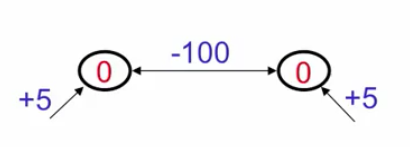
\includegraphics[scale=0.9]{sections/11/osc.png}
		\end{center}
		\item At the next parllel step, both units will turn on. This has very high energy, so then they will both turn off again.
	\end{itemize}

	\item If the updates occur in parallel but with random timing, the oscillations are usually destroyed
	
	\subsubsection{A neat way to make use of this type of computation}
	\item Hopfield proposed that memories could be energy minima of a neural net
	\begin{itemize}
		\item The binary threshold decision rule can then be used to ``clean up'' incomplete or corrupted memories
	\end{itemize}
	\item The idea of memories as energy minima was proposed by I.A. Richards in 1924 in ``Principles of Literary Criticism''
	\item Using energy minima to represent memories gives a content-adressable memory
	\begin{itemize}
		\item An item can be assessed by just knowing part of its content
		\item It is robust against hardware damage
		\item It's like reconstructing a dinosaur from a few bones
	\end{itemize}

	\subsubsection{Storing memories in a Hopfield net}
	\item If we use activities of 1 and -1, we can store a binary state vector by incrementing the weight between any two units by the product of their activities.
		$$\delta w_{ij} = s_i s_j$$
	\item This is a very simple rule that is not error-driven.That is both its strenght and its weakness. 
	\item We treat biases as weights from a permanently on unit
	\item With states of 0 and 1 the rule is slightly more complicated:
		$$\delta w_{ij} = 4(s_i - \frac{1}{2})(s_j - \frac{1}{2})$$
\end{itemize}